%%%%%%%%%%%%%%%%%%%%%%%%%%%%%%%%%%%%%%%%%%%%%%%%%%%%%%%%%%%%%%%%%%%%%%%%%%%%%%%%%%
\begin{frame}[fragile]\frametitle{}

\begin{center}
{\Large NER with Conditional Random Fields (CRF)}

{\tiny (Ref:C omplete Tutorial on Named Entity Recognition (NER) using Python and Keras - by Akshay Chavan)}
\end{center}


\end{frame}

%%%%%%%%%%%%%%%%%%%%%%%%%%%%%%%%%%%%%%%%%%%%%%%%%%%%%%%%%%%%%%%%%%%%%%%%%%%%%%%%%%
\begin{frame}[fragile]\frametitle{Conditional Random Fields (CRFs)}
  \begin{itemize}
  \item CRFs are used for predicting the sequences that use the contextual information to add information which will be used by the model to make a correct prediction.
	\item The output sequence is modeled as the normalized product of the feature function.
	\item Actually its similar to basic Logistic Regression, done for each token, with a custom feature lists, having info of the context.
  \end{itemize}
	
	\begin{center}
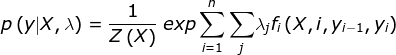
\includegraphics[width=0.5\linewidth,keepaspectratio]{ner13}
\end{center}
\end{frame}



% %%%%%%%%%%%%%%%%%%%%%%%%%%%%%%%%%%%%%%%%%%%%%%%%%%%%%%%%%%%%%%%%%%%%%%%%%%%%%%%%%%
% \begin{frame}[fragile]\frametitle{NER}
% NER is a method of extracting the relevant information from a large corpus and classifying those entities into predefined categories such as location, organization, name and so on. 
	
% \begin{center}
% 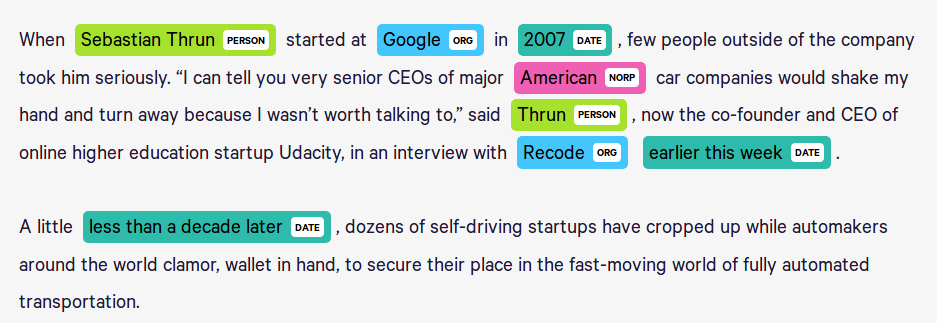
\includegraphics[width=0.8\linewidth,keepaspectratio]{spacy18}

	% {\tiny (Ref: Complete Tutorial on Named Entity Recognition (NER) using Python and Keras - by Akshay Chavan)}

% \end{center}

% The conditional random field is used for predicting the sequences that use the contextual information to add information which will be used by the model to make correct predictions.

	% {\tiny (Ref: Introduction to Conditional Random Fields (CRFs) - by Akshay Chavan)}

% \end{frame}

%%%%%%%%%%%%%%%%%%%%%%%%%%%%%%%%%%%%%%%%%%%%%%%%%%%%%%%%%%%%%%%%%%%%%%%%%%%%%%%%%%
\begin{frame}[fragile]\frametitle{CRFs}
  \begin{itemize}
  \item To predict an output vector $y = {y_0, y_1, \ldots y_n}$ of a random variable given a feature vector $X$.
	\item The goal is to not only predict the output vector correctly but also the sequence of predictions matter a lot.
	\item The model predicts many variables that are interdependent.
	\item The main challenge behind the NER problem is that the entities that are too rare to appear in training set due to which model must identify based only on context. 
	\item The naive approach to this problem is to classify each word independently. 
	\item The main problem with this approach is it assumes that named entity labels are independent which is not the case.
	\item In CRFs where input data is sequence and output is also a sequence and we have to take the previous context into account when predicting on a data point.
  \end{itemize}
	

\end{frame}


%%%%%%%%%%%%%%%%%%%%%%%%%%%%%%%%%%%%%%%%%%%%%%%%%%%%%%%%%%%%%%%%%%%%%%%%%%%%%%%%%%
\begin{frame}[fragile]\frametitle{Sequence Modeling  CRF}

\begin{center}
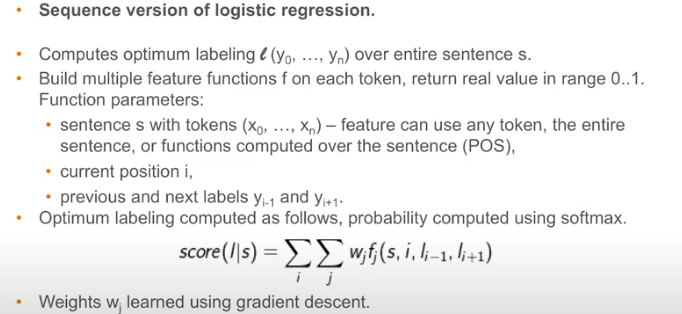
\includegraphics[width=\linewidth,keepaspectratio]{ner19}
\end{center}

{\tiny (Ref: Sujit Pal: Building Named Entity Recognition Models Efficiently Using NERDS | PyData LA 2019)}

\end{frame}


%%%%%%%%%%%%%%%%%%%%%%%%%%%%%%%%%%%%%%%%%%%%%%%%%%%%%%%%%%%%%%%%%%%%%%%%%%%%%%%%%%
\begin{frame}[fragile]\frametitle{}

\begin{center}
{\Large Test case}
\end{center}
\end{frame}

%%%%%%%%%%%%%%%%%%%%%%%%%%%%%%%%%%%%%%%%%%%%%%%%%%%%%%%%%%%%%%%%%%%%%%%%%%%%%%%%%%
\begin{frame}[fragile]\frametitle{Understanding the data}

Source: https://www.kaggle.com/abhinavwalia95/entity-annotated-corpus having GMB(Groningen Meaning Bank) corpus which is tagged, annotated and built specifically to train the classifier to predict named entities such as name, location, etc. in BIO (or IOB) format where  B- denotes the beginning and I- inside of an entity. The words which are not of interest are labeled with 0 – tag.

\begin{lstlisting}
df = pd.read_csv('ner_dataset.csv', encoding = "ISO-8859-1")
print(df.head(10))
\end{lstlisting}


\begin{center}
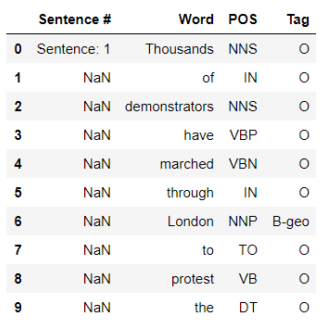
\includegraphics[width=0.4\linewidth,keepaspectratio]{spacy19}
\end{center}

\end{frame}




%%%%%%%%%%%%%%%%%%%%%%%%%%%%%%%%%%%%%%%%%%%%%%%%%%%%%%%%%%%%%%%%%%%%%%%%%%%%%%%%%%
\begin{frame}[fragile]\frametitle{Labels}
  \begin{itemize}
  \item geo = Geographical Entity
  \item org = Organization
  \item per = Person
  \item gpe = Geopolitical Entity
  \item tim = Time indicator
  \item art = Artifact
  \item eve = Event
  \item nat = Natural Phenomenon
  \end{itemize}
	

\end{frame}

%%%%%%%%%%%%%%%%%%%%%%%%%%%%%%%%%%%%%%%%%%%%%%%%%%%%%%%%%%%%%%%%%%%%%%%%%%%%%%%%%%
\begin{frame}[fragile]\frametitle{Understanding the data}


\begin{lstlisting}
df.describe()
\end{lstlisting}

\begin{center}
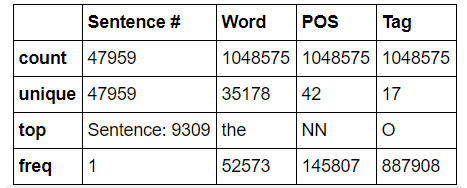
\includegraphics[width=0.35\linewidth,keepaspectratio]{spacy20}
\end{center}

\begin{lstlisting}
df['Tag'].unique()
array(['O', 'B-geo', 'B-gpe', 'B-per', 'I-geo', 'B-org', 'I-org', 'B-tim',
       'B-art', 'I-art', 'I-per', 'I-gpe', 'I-tim', 'B-nat', 'B-eve',
       'I-eve', 'I-nat'], dtype=object)
			 
df.isnull().sum()
Sentence #    1000616
Word                0
POS                 0
Tag                 0
\end{lstlisting}

  \begin{itemize}
  \item Total 47959 sentences and 17 labels.
  \item Number unique words in the dataset are 35178.
	\item Lots of missing values in 'Sentence \#' attribute.
  \end{itemize}
\end{frame}

%%%%%%%%%%%%%%%%%%%%%%%%%%%%%%%%%%%%%%%%%%%%%%%%%%%%%%%%%%%%%%%%%%%%%%%%%%%%%%%%%%
\begin{frame}[fragile]\frametitle{Preprocessing the data}

Populate sentences objects. Each will be list of tuples with its tag and pos.

\begin{lstlisting}
class sentence(object):
    def __init__(self, df):
        self.n_sent = 1
        self.df = df
        self.empty = False
        agg = lambda s : [(w, p, t) for w, p, t in zip(s['Word'].values.tolist(),
                                                       s['POS'].values.tolist(),
                                                       s['Tag'].values.tolist())]
        self.grouped = self.df.groupby("Sentence #").apply(agg)
        self.sentences = [s for s in self.grouped]
        
    def get_text(self):
        try:
            s = self.grouped['Sentence: {}'.format(self.n_sent)]
            self.n_sent +=1
            return s
        except:
            return None
\end{lstlisting}
\end{frame}

%%%%%%%%%%%%%%%%%%%%%%%%%%%%%%%%%%%%%%%%%%%%%%%%%%%%%%%%%%%%%%%%%%%%%%%%%%%%%%%%%%
\begin{frame}[fragile]\frametitle{Preprocessing the data}


\begin{lstlisting}
getter = sentence(df)
sent = getter.get_text()
print(sent)

[('Thousands', 'NNS', 'O'), ('of', 'IN', 'O'), ('demonstrators', 'NNS', 'O'), ('have', 'VBP', 'O'), ('marched', 'VBN', 'O'), ('through', 'IN', 'O'), ('London', 'NNP', 'B-geo'), ('to', 'TO', 'O'), ('protest', 'VB', 'O'), ('the', 'DT', 'O'), ('war', 'NN', 'O'), ('in', 'IN', 'O'), ('Iraq', 'NNP', 'B-geo'), ('and', 'CC', 'O'), ('demand', 'VB', 'O'), ('the', 'DT', 'O'), ('withdrawal', 'NN', 'O'), ('of', 'IN', 'O'), ('British', 'JJ', 'B-gpe'), ('troops', 'NNS', 'O'), ('from', 'IN', 'O'), ('that', 'DT', 'O'), ('country', 'NN', 'O'), ('.', '.', 'O')]

# Getting all the sentences in the dataset.
sentences = [" ".join([s[0] for s in sent]) for sent in getter.sentences]

\end{lstlisting}
\end{frame}

%%%%%%%%%%%%%%%%%%%%%%%%%%%%%%%%%%%%%%%%%%%%%%%%%%%%%%%%%%%%%%%%%%%%%%%%%%%%%%%%%%
\begin{frame}[fragile]\frametitle{Feature Preparation}


\begin{lstlisting}
def word2features(sent, i):
    word = sent[i][0]
    postag = sent[i][1]
    features = {
        'bias': 1.0,
        'word.lower()': word.lower(),
        'word[-3:]': word[-3:],
        'word[-2:]': word[-2:],
        'word.isupper()': word.isupper(),
        'word.istitle()': word.istitle(),
        'word.isdigit()': word.isdigit(),
        'postag': postag,
        'postag[:2]': postag[:2],
    }
    if i > 0:
        word1 = sent[i-1][0]
        postag1 = sent[i-1][1]
        features.update({
            '-1:word.lower()': word1.lower(),
            '-1:word.istitle()': word1.istitle(),
            '-1:word.isupper()': word1.isupper(),
            '-1:postag': postag1,
            '-1:postag[:2]': postag1[:2]})
    else:
        features['BOS'] = True
\end{lstlisting}
\end{frame}

%%%%%%%%%%%%%%%%%%%%%%%%%%%%%%%%%%%%%%%%%%%%%%%%%%%%%%%%%%%%%%%%%%%%%%%%%%%%%%%%%%
\begin{frame}[fragile]\frametitle{Feature Preparation}


\begin{lstlisting}
def word2features(sent, i):
		:
    if i < len(sent)-1:
        word1 = sent[i+1][0]
        postag1 = sent[i+1][1]
        features.update({
            '+1:word.lower()': word1.lower(),
            '+1:word.istitle()': word1.istitle(),
            '+1:word.isupper()': word1.isupper(),
            '+1:postag': postag1,
            '+1:postag[:2]': postag1[:2],
        })
    else:
        features['EOS'] = True
    return features
		
def sent2features(sent):
    return [word2features(sent, i) for i in range(len(sent))]
def sent2labels(sent):
    return [label for token, postag, label in sent]
def sent2tokens(sent):
    return [token for token, postag, label in sent]		
\end{lstlisting}
\end{frame}

%%%%%%%%%%%%%%%%%%%%%%%%%%%%%%%%%%%%%%%%%%%%%%%%%%%%%%%%%%%%%%%%%%%%%%%%%%%%%%%%%%
\begin{frame}[fragile]\frametitle{Training}


\begin{lstlisting}
X = [sent2features(s) for s in sentences]
y = [sent2labels(s) for s in sentences]
X_train, X_test, y_train, y_test = train_test_split(X, y, test_size = 0.2)

crf = CRF(algorithm = 'lbfgs',
         c1 = 0.1,
         c2 = 0.1,
         max_iterations = 100,
         all_possible_transitions = False)
crf.fit(X_train, y_train)
y_pred = crf.predict(X_test)
\end{lstlisting}
\end{frame}

%%%%%%%%%%%%%%%%%%%%%%%%%%%%%%%%%%%%%%%%%%%%%%%%%%%%%%%%%%%%%%%%%%%%%%%%%%%%%%%%%%
\begin{frame}[fragile]\frametitle{Evaluating}
\begin{lstlisting}
f1_score = flat_f1_score(y_test, y_pred, average = 'weighted')
0.9719578426137272
report = flat_classification_report(y_test, y_pred)
             precision    recall  f1-score   support
      B-art       0.43      0.17      0.24        78
      B-eve       0.68      0.41      0.51        61
      B-geo       0.86      0.91      0.88      7481
      B-gpe       0.97      0.94      0.95      3185
      B-nat       0.85      0.36      0.51        47
      B-org       0.81      0.74      0.77      4187
      B-per       0.86      0.83      0.84      3421
      B-tim       0.93      0.88      0.90      4030
      I-art       0.25      0.08      0.12        64
      I-eve       0.52      0.30      0.38        44
      I-geo       0.81      0.80      0.80      1461
      I-gpe       0.81      0.46      0.59        37
      I-nat       0.50      0.17      0.25        12
      I-org       0.83      0.81      0.82      3441
      I-per       0.86      0.90      0.88      3488
      I-tim       0.84      0.74      0.79      1245
          O       0.99      0.99      0.99    177951
avg / total       0.97      0.97      0.97    210233
\end{lstlisting}

Good results!!
\end{frame}